% ##################################################################################################################
\section{Patna, India}
\label{sec:patna}
\hfill \textbf{Author:} Amit Agarwal

% ##################################################################################################################
Patna is a medium sized city in eastern part of India. Similar to other developing nations, in Patna also, traffic conditions are heterogeneous due to presence of significantly higher number of motorized (motorbike, 14\,\%) and non-motorized (bike, 33\,\%) vehicles than car (only 2\,\%). Therefore, the MATSim queue simulation is modified to simulate travel demand under mixed traffic conditions.

The Patna scenario is created using household survey data from comprehensive mobility plan for Patna \citep[][]{TrippItransVks2009PatnaReport}. To create the Patna scenario, the area under Patna Municipal Corporation is used. The scenario is composed of 72\,zones with a population of about 1.57\,million (year 2008). In this scenario, MATSim demand is generated using trip diaries. Car, motorbike and bike are used as main congested modes (Figure~\ref{fig:patna0}). Passenger car unit for vehicles is derived using effective area occupied by vehicles. In order to allow overtaking of slower vehicles (bike) by faster vehicles (car and motorbike), preexisting, state-of-the-art FIFO (first-in-first-out) queue simulation is overridden using earliest link exit time as shown in Figure~\ref{fig:patna1}. Detailed description of the scenario can be found in \citet[][]{AgarwalEtcMixedTraffic}.

Later, the behavior of traffic ow in modified queue simulation is analyzed by plotting fundamental diagrams and space time trajectories for car, motorbike and bike.

\createfigure%
{Patna: Various vehicles on network, car in red, motorbike in blue and bike in green}%
{Patna: Various vehicles on network, car in red, motorbike in blue and bike in green}%
{\label{fig:patna0}}%
{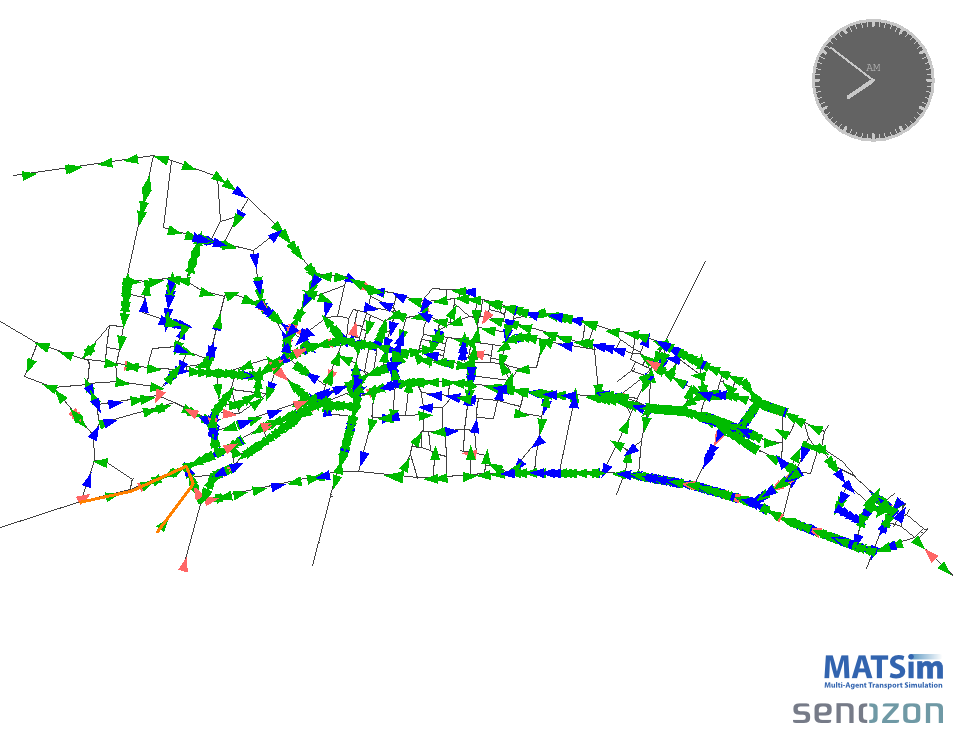
\includegraphics[width=0.99\textwidth, angle=0]{using/figures/vehiclesOnNetwork}}%
{}

\createfigure%
{Patna: FIFO Approach and passing of bicycle by car on a link (not to scale)}%
{Patna: FIFO Approach and passing of bicycle by car on a link (not to scale)}%
{\label{fig:patna1}}%
{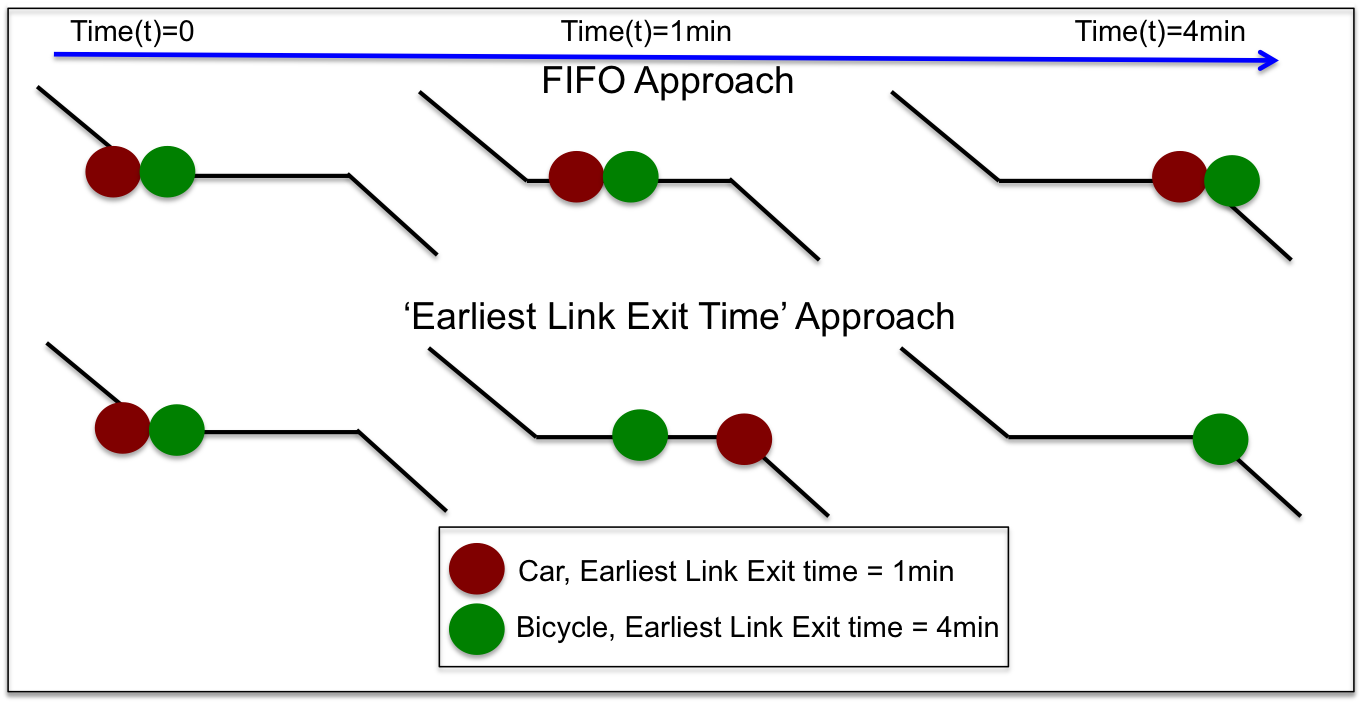
\includegraphics[width=0.99\textwidth, angle=0]{using/figures/FIFOandPassing}}%
{}

% ##################################################################################################################